\chapter{Bewertung}
In diesem Kapitel wird das im vorherigen Kapitel beschriebene System beurteilt und mit dem vorhergehenden System verglichen.
Aufgrund der sich unterscheidenden Infrastrukturen der beiden Systeme, ist es nicht möglich einen direkten Vergleich durchzuführen.
Stattdessen müssen verschiedene Kennzahlen bezüglich der zu erfüllenden Anforderungen gefunden werden, um einen Vergleich zwischen den Kennzahlen des jeweiligen Systems durchzuführen.

\section{Abweichungen der Systeme}
Das in dieser Arbeit beschriebene System wurde besonders im Hinblick auf Ressourceneffizienz optimiert.
Somit gibt es auch starke Unterscheidungen zum alten System, welches lediglich ergebnisorientiert entworfen wurde und daher einen erhöhten Ressourcenverbrauch besitzt.

Um weniger Ressourcen zu verbrauchen, wurde zum einen auch die Auswertung von Verkehrskamerabildern vereinfacht.
Statt der Verwendung eines neuronalen Netzes, welches einen sehr hohen Ressourcenbedarf mit sich zieht, wird nun ein weniger komplexer Background-Subtraction Algorithmus verwendet.

Die Auswertung wird dadurch so stark vereinigt, dass sie sich auch auf die Clients auslagern lässt.
Das Backend kann also als einfacher Zwischenspeicher für Daten der Straßenverkehrszentrale Baden-Württemberg verwendet werden und ist somit auch für den Nutzen auf einem Shared-Webhost optimiert.

Durch die Auslagerung der Auswertung auf die Clients ist jedoch auch nun der Großteil der Berechnung auf dem Client zu finden.
Es ist daher wichtig bestimmte Kenngrößen zu finden, um das eher client-lastige neue System mit dem server-lastigen Altsystem zu vergleichen.

\section{Kennzahlen}
Wichtige Kennzahlen für den Vergleich zwischen Neu- und Altsystem sollten vor allem die Anforderungen an das System widerspiegeln.
So ist es sinnvoll, auch die während der Laufzeit benötigten Ressourcen zu messen, sowie die Genauigkeit des Systems zu bestimmen.
Während der Arbeit wurden folgende Kennzahlen zum Vergleich der Systeme bestimmt:
\begin{itemize}
\item{Arbeitsspeicher-Last des Systems}
\item{CPU-Last des jeweiligen Servers}
\item{Energieverbrauch des Clients}
\item{Genauigkeit des Systems}
\end{itemize}
Wobei die Arbeitsspeicher-Last des gesamten Systems jeweils am Client und am Server gemessen werden muss.

Diese Arbeit befasst sich aufgrund der Aufgabenstellung hauptsächlich mit der Optimierung der Arbeitsspeicher-Last.
Diese Ressource ist dabei auch eine der Ressourcen, welche kritisch für die Funktionalität des Systems sind.
Wenn das System an die Arbeitsspeichergrenze kommen würde, könnte dies bedeuten, dass die Applikation frühzeitig beendet wird oder erst gar nicht starten kann.
Wohingegen Energieverbrauch und CPU-Last meist nicht an konkrete Limitierungen gebunden sind.

\paragraph*{Nicht berücksichtigte Kennzahlen}

Da Sekundärspeicher in der heutigen Zeit relativ günstig ist und das System keinen hohen Gebrauch des Speichers macht, wurde dieser nicht für den Vergleich gemessen.
Ebenfalls wurde die Auswirkung von mehreren Clients auf die Ressourcen-Last nicht berücksichtigt, da das System in der Zielumgebung keine großen Nutzermengen unterstützen muss.
\newpage

\section{Datenerhebung}
Die beschriebenen Kennzahlen müssen nun zur Laufzeit im jeweiligen System gemessen werden.
Hierzu stehen verschiedene Methoden und Programme zur Verfügung, welche das Messen der jeweiligen Kenngröße ermöglichen.
Im folgenden wird die für die Arbeit angemessene Herangehensweise beschrieben, um die jeweilige Kennzahl während der Laufzeit zu messen.\newline\newline
\textbf{Arbeitsspeicher-Last des Systems}\newline
Die Arbeitsspeicher-Last des Systems gilt an zwei Stellen zu messen: am Client und am Server.
Für die Messung der Arbeitsspeicher-Last am Server wurde zur Laufzeit das Programm "`htop"' verwendet.
htop ist dabei ein Programm welches auf dem Linux Betriebssystem installiert werden kann und eine Übersicht der derzeit laufende Prozesse bietet.
Zusätzlich werden auch alle belegten Systemressourcen für die jeweiligen Prozesse angegeben.\newline\newline
\textbf{CPU-Last des Servers}\newline
Die CPU-Last des Servers lässt sich ebenfalls über das Programm htop ermitteln. 
Da die CPU-Last während der Laufzeit jedoch stark schwankt, macht es mehr Sinn hierfür einen Mittelwert über die Laufzeit zu erstellen.\newline\newline
\textbf{Energieverbrauch des Clients}\newline
Der Energieverbrauch des Clients lässt sich über die Profiler-Ansicht von Android Studio ermitteln.
Der sogenannte "`Energy Profiler"' überwacht dabei zusätzlich zur CPU auch andere Peripheriegeräte, wie zum Beispiel den eingebauten GPS Sensor in dem jeweiligen Smartphone.
Weiterhin werden auch System-Events, wie Alarme, Jobs oder Ortungsanfragen analysiert, welche ebenfalls den Energieverbrauch einer App beeinflussen können.\newline\newline
%\textbf{Genauigkeit des Systems}\newline
%Needed?...

\newpage


\section{Auswertung}
\subsection{Backend}
\begin{figure}[ht]
   \centering
     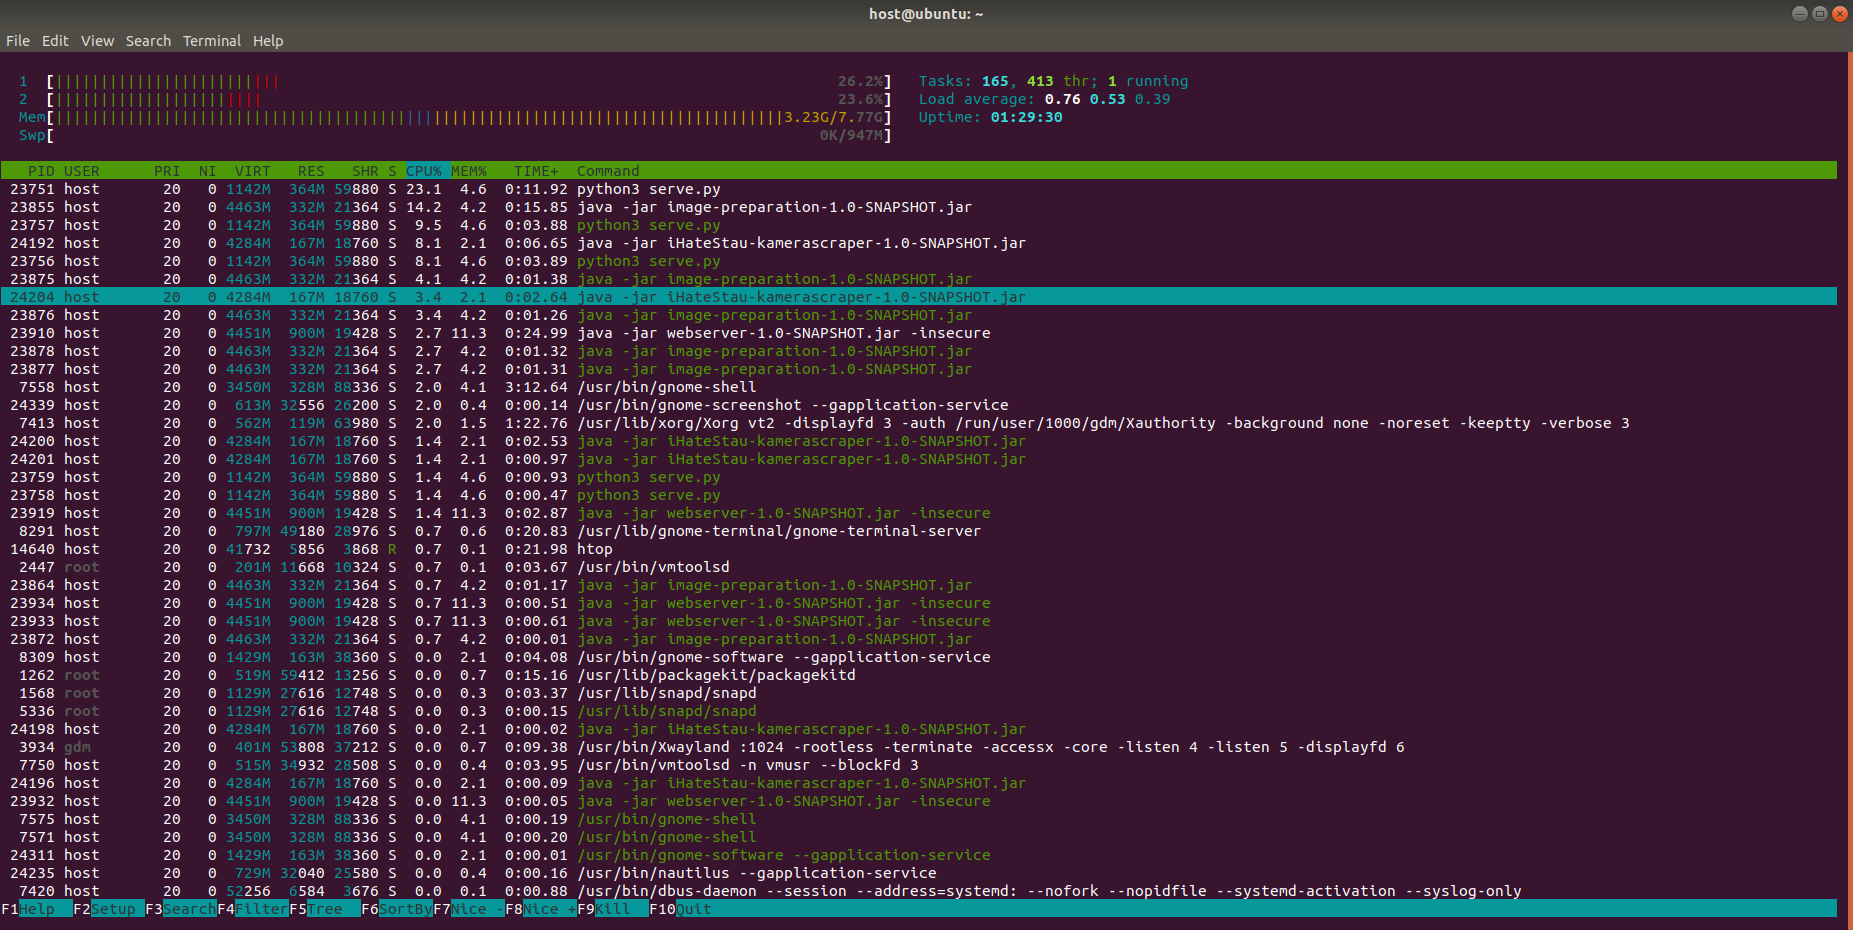
\includegraphics[width=15cm]{Bilder/server-ihatestau} \\
 \caption{Ressourcenverbrauch alter Server in htop}
 \label{fig:ihatestau-res}
\end{figure}
\begin{figure}[ht]
   \centering
     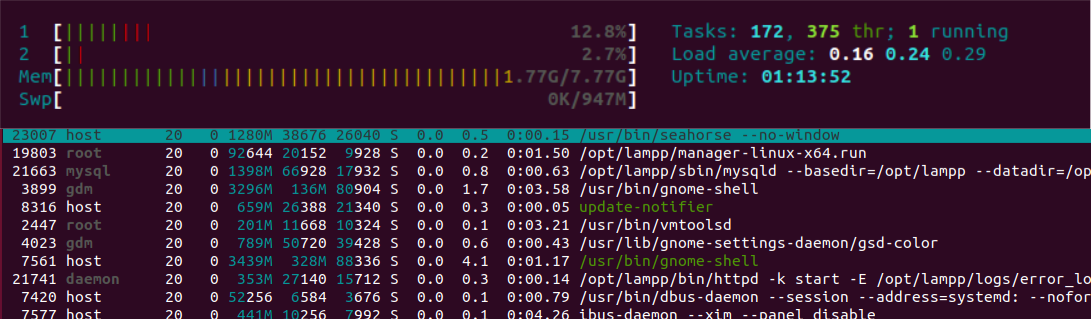
\includegraphics[width=15cm]{Bilder/server-new} \\
 \caption{Ressourcenverbrauch neuer Server in htop}
 \label{fig:new-server-res}
\end{figure}

Auf den Abbildungen~\ref{fig:ihatestau-res} und~\ref{fig:new-server-res} wird der Arbeitsspeicher- und CPU-Nutzungsbedarf des alten und neuen Backends visualisiert.

Bei dem Anblick der Abbildung wird auch klar, dass das alte System eher auf ein Anwendungsszenario im Großbetrieb ausgelegt war, da es sehr starken Gebrauch von Nebenläufigkeit und mehreren Threads macht.
Dies ist für ein Szenario in dem sehr viele Benutzer unterstützt werden sollen durchaus sinnvoll.
Jedoch bedeutet dies auch, dass das System einen hohen initialen Bedarf an Ressourcen hat, der sich pro Benutzer auch noch steigert.
In der Abbildung~\ref{fig:new-server-res} sieht man daher nur wenige Prozesse und keine Threads, die explizit von dem System verwendet werden.
Somit ist der Ressourcenverbrauch beim Starten des Systems stark reduziert.

Weiterhin werden auch weniger Ressourcen pro Benutzer benötigt.
Was hier jedoch ganz klar ein Nachteil im neuen System darstellt, ist, dass es nicht mehr für große Nutzermengen ausgelegt ist.
Es nutzt keine Skalierungsmaßnahmen wie Threads und Nebenläufigkeit aus und kann daher leicht bei großen Nutzerzahlen an die Systemgrenzen stoßen.

Diese Arbeit konzentriert sich auf den Betrieb des Backends für eine sehr kleine Nutzermenge, daher ist dieser Nachteil für das Ergebnis unerheblich.

\subsection{Frontend}
\begin{figure}[ht]
  \centering
	\begin{minipage}[b]{0.4\textwidth}
     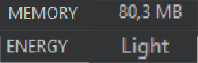
\includegraphics[width=\textwidth]{Bilder/res-app-old} \\
   \caption{Ressourcenverbrauch alter Client}
   \label{fig:res-app-old}
  \end{minipage}
	\hfill
	\begin{minipage}[b]{0.4\textwidth}
     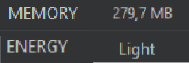
\includegraphics[width=\textwidth]{Bilder/res-app-new} \\
		\caption{Ressourcenverbrauch neuer Client}
		\label{fig:res-app-new}
	\end{minipage}
\end{figure}

Abbildung~\ref{fig:res-app-new} visualisiert einen Anstieg des Arbeitsspeicher-Verbrauchs im Vergleich zum alten Client, dessen Kennzahlen auf Abbildung~\ref{fig:res-app-old} zu sehen sind.
Dabei handelt es sich fast um eine Vervierfachung des ursprünglichen Arbeitsspeicherbedarfs.
Dies lässt sich natürlich vor allem durch die client-seitige Auswertung von Bildern erklären, da der hierfür benötigte Algorithmus mehrere Bilder im Arbeitsspeicher behält (siehe Abschnitt~\ref{sec:backsub-algo}).
Jedoch befindet sich der Arbeitsspeicherbedarf, selbst beim neuen Client, immer noch unter einem halben Gigabyte.

Mit den derzeitigen Hardware-Standards für Smartphones lässt sich dies gut vereinbaren, da aktuelle Smartphones bereits über mehrere Gigabytes an Arbeitsspeicher besitzen.
So lassen sich auch andere Applikationen parallel zur Verwendung des Clients nutzen.
Die Android Applikation "`YouTube"' benötigt beispielsweise ebenfalls etwa einen halben Gigabyte an Arbeitspeicher bei Benutzung.

Der Energiebedarf des neuen Clients ist laut dem Energy Profiler von Android Studio im Vergleich zum alten System gleich geblieben.
Dies lässt sich durch die wenigen Anfragen erklären, die der Client im Vergleich zum alten System tätigen muss.
Da der Client in einer Anfrage an das Backend direkt alle nötigten Bilder gesendet bekommt, muss er nicht einzeln anfragen.
Weiterhin verwendet der neue Client keine Google-APIs mehr, welche auch zusätzlichen Energiebedarf mit sich bringen.

Der gezeigte Wert für den Energieverbrauch ist jedoch nur gemittelt und als Rangmerkmal beschrieben, so kann es sein dass einzelne Ausreißer im Energieverbrauch der Applikation existieren. Um diese Ausreißer festzustellen, müsste jedoch eine konkrete Analyse der Applikation auf dem Betriebssystem des Smartphones stattfinden, welche im Rahmen dieser Arbeit übersprungen wurde.
